% !TeX spellcheck = en_US
\addscenariosection[subsection]{1}{Campaign name}{Scenario name}{\images/title.png}

\begin{multicols*}{2}

\textbf{Author:} ...

\textbf{Source:} ...

\subsection*{\MakeUppercase{Scenario length}}

This scenario plays out over ... Rounds.

\subsection*{\MakeUppercase{Player setup}}

\textbf{Faction:} ...

\textbf{Faction Hero:} ...

\textbf{Starting Resources:} X \svg{gold}, Y \svg{building_materials}, Z \svg{valuables}

\textbf{Starting Income:} A \svg{gold}, B \svg{building_materials}, C \svg{valuables}

\textbf{Starting Units:}
\begin{itemize}
  \item A Few \svgunit{bronze}...
  \item A Pack \svgunit{silver}...
  \item \svgunit{golden}
  \item \svg{azure}
\end{itemize}

\textbf{Town Buildings:} \svgunit{bronze} Dwelling...

\textbf{Bonus:} Choose one of the following options:
\begin{itemize}
    \item ...
\end{itemize}

\subsection*{\MakeUppercase{AI hero setup}}

\textbf{Faction:} ...

\textbf{Enemy Army:} ...

\textbf{Enemy Deck:} ...

\textbf{Enemy Spell Deck:} ...

\textbf{Enemy Skills:} ...

\textbf{Special:} ...

\subsection*{\MakeUppercase{Map setup}}

Take the following Map Tiles and arrange them as shown in the scenario map layout:

\textbf{X × Starting (I) Map Tile}
\begin{itemize}
    \item ... additional constraints ...
\end{itemize}

\textbf{Y × Far (II--III) Map Tile}

\textbf{Z × Near (IV--V) Map Tile}

\subsection*{\MakeUppercase{Heroes placement}}

... describe how your and enemy heroes will be placed ...

\subsection*{\MakeUppercase{Victory Conditions}}
...

\subsection*{\MakeUppercase{Defeat Conditions}}
...

\subsection*{\MakeUppercase{Timed Events}}

% Unless you have a rich and non-linear story, write it under specific
% Rounds here.
%
% Otherwise create a new subsection "The Story" at the end and refer to it.

\textbf{\nth{2} Round:}
\begin{itemize}
  \item ...
  \item ...
\end{itemize}

% IF THERE ARE OVERLAPPING EVENTS, FOLLOW BELOW STRUCTURE, IN CHRONOLOGICAL ORDER
%
% \textbf{\nth{7} and \nth{8} Rounds:}
% \begin{itemize}
%   \item ...
% \end{itemize}
%
% \textbf{\nth{9} Round:}
% \begin{itemize}
%   \item Repeat Timed Events of Round 6.
% \end{itemize}
%
% \textbf{\nth{10} Round:}
% \begin{itemize}
%   \item Repeat Timed Events of Rounds 7 and 8.
% \end{itemize}

\subsection*{\MakeUppercase{Additional rules}}

During this ``... Faction ...'' Campaign scenario, the following rules apply:

\begin{itemize}
  \item ...
\end{itemize}

\end{multicols*}

\newpage

% NOTE: The last page of scenario preparation should use
% multicols instead of multicols* to create space for map.
% \begin{multicols}{2}
% ... your content that overflows to the second page ...
% \end{multicols}

% Uncomment and link a map image
% \vspace{3em}
% \begin{center}
%   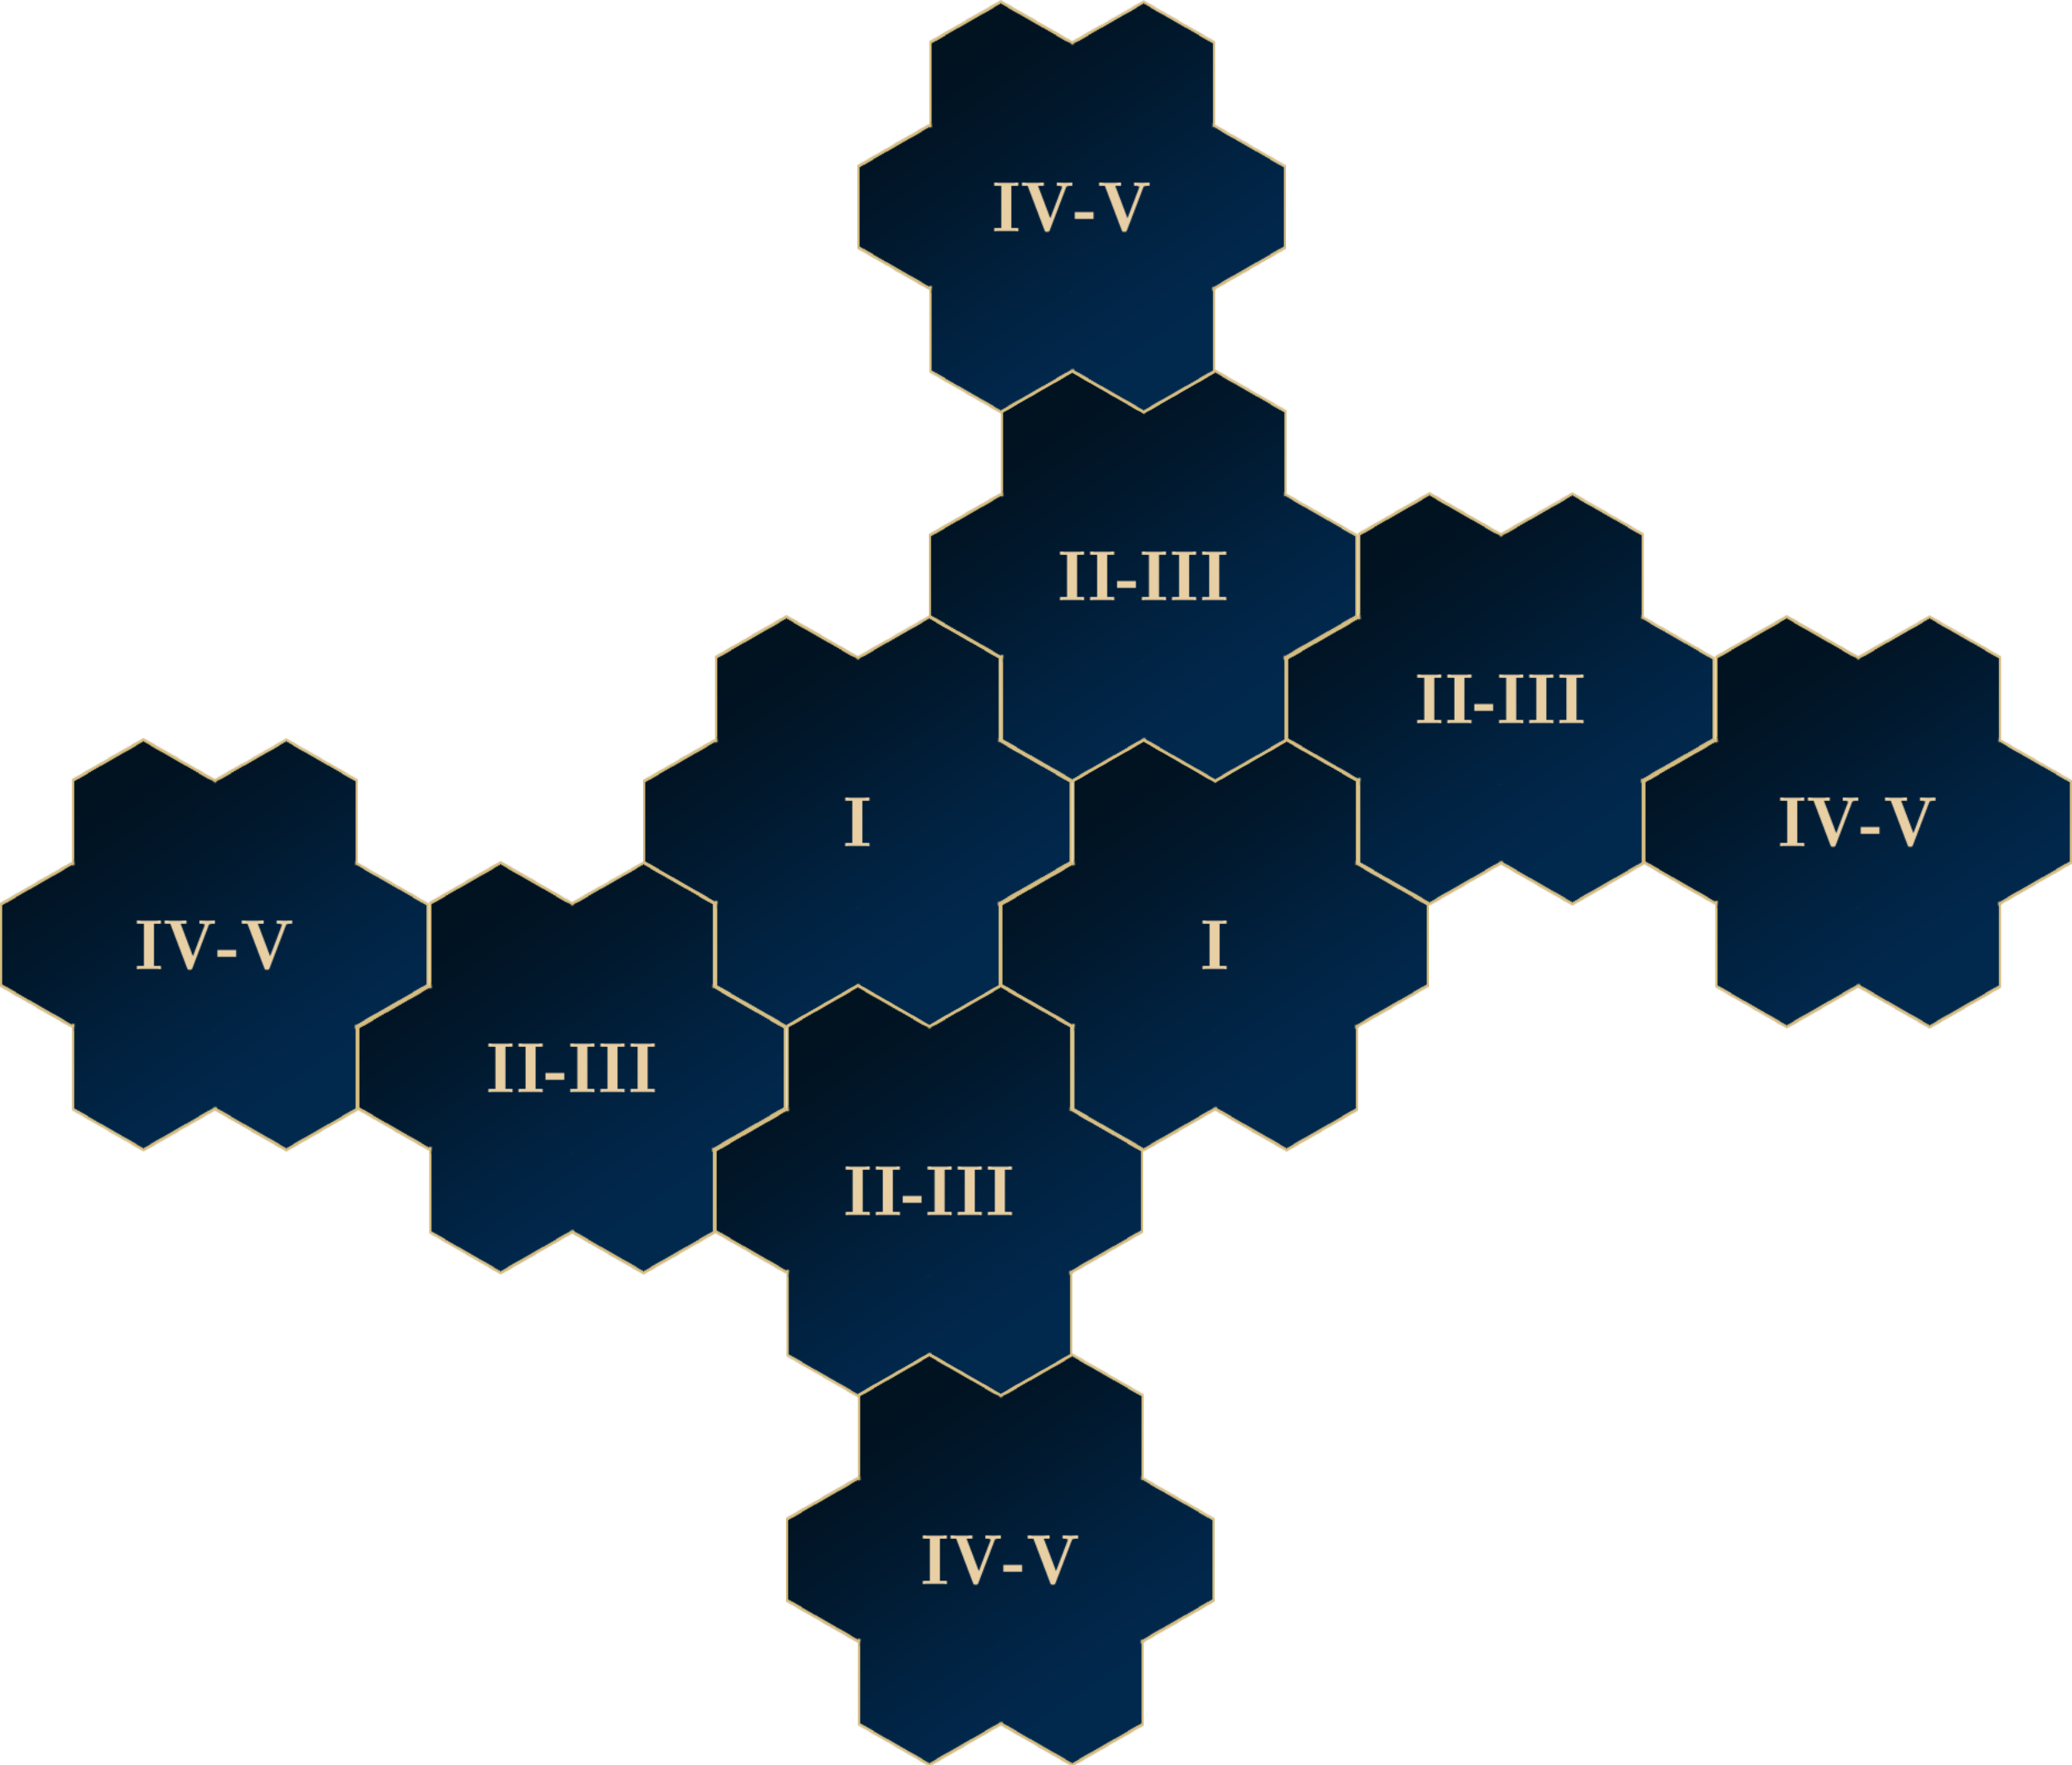
\includegraphics[width=0.6\paperwidth]{\_assets/maps/sentinels.png}
% \end{center}

\newpage

\begin{multicols*}{2}

\subsection*{\MakeUppercase{The story}}

... put your immersive story here ...

\end{multicols*}
